% Relatório  para Disciplina de Controle Fuzzy - UFRN
% Autores:

%   DANIEL HENRIQUE SILVA FERNANDES
%   FERNANDO LEANDRO FERNANDES
%   ROSENILDO PEREIRA AGUIAR FURTADO
%   TIAGO BATISTA SILVA SOUSA 

%%%%%%%%%%%%%%%%%%%%%%%% STRUCTURE %%%%%%%%%%%%%%%%%%%%%%%%%%
\documentclass[a4paper,12pt]{article}
\usepackage[T1]{fontenc}
\usepackage[utf8]{inputenc}
\usepackage[brazil]{babel}
\usepackage{lmodern}
\usepackage{setspace}
\usepackage[top=2cm, bottom=2cm, left=2cm, right=2cm]{geometry}
\usepackage{indentfirst} 


%%%%%%%%%%%%%%%%%%%%%%%%%%%% PAGES STYLE %%%%%%%%%%%%%%%%%%%%%
\usepackage{fancyhdr}
\fancypagestyle{main}{
\renewcommand{\headrulewidth}{0pt}
\fancyhead[RO]{\thepage}
\fancyfoot[CO]{}
}
%%%%%%%%%%%%%%%%%%%%%%  PACOTES  %%%%%%%%%%%%%%%%%%%%%%%%%%%%

\usepackage{graphicx}
\usepackage{epstopdf}
\usepackage{subfig}
\usepackage{mathptmx}
\usepackage{changepage}
\usepackage{amsmath}
%\usepackage[alf]{abntex2cite}


%%%%%%%%%%%%%%%%%%%%%%% PDF METADATA %%%%%%%%%%%%%%%%%%%%%%%%%

\usepackage[ pdftitle={6 Relatório SC},
pdfsubject={CONTROLE NO ESPAÇO DE ESTADOS: SEGUIDOR DE REFERÊNCIA - Grupo 1},
pdfkeywords={Controle,Automação,UFRN,DCA,ipump},
hidelinks]{hyperref}

%%%%%%%%%%%%% Criando novo tipo de lista %%%%%%%%%%%%%%%%%%%%%%
% http://texblog.org/2008/07/13/define-your-own-list-of/

\usepackage{tocloft}
\newcommand{\listexamplename}{Lista de Equações}
\newlistof{equacao}{exp}{\listexamplename}
\newcommand{\equacao}[1] {%
    \refstepcounter{equacao}
    \par\noindent\begin{center}\textbf{Equação \theequacao. #1}\end{center}
    \addcontentsline{exp}{equacao}
        {\protect\numberline{\thesection.\theequacao}\quad#1}\par
}


%%%%%%%%%%%%% Criando novo tipo de lista %%%%%%%%%%%%%%%%%%%%%%



%%%%%%%%%%%%%%%%%%%%%%%%%%%%%%%%%%%%%%%%%%%%%%%%%%%%%%%%%%%%%%%%%

\begin{document}

\onehalfspacing

\thispagestyle{empty}

\setcounter{page}{1}

%%%%%%%%%%%%%%%%%%%%%%% LOGOS %%%%%%%%%%%%%%%%%%%%%%%%%%%%%%%

\begin{figure}[!ht]

\centering

\subfloat{
\includegraphics[width=2.7cm]{Imagens/UFRN.eps}
\label{UFRN Logo}
}
\hspace{11.09cm}
\subfloat{

\includegraphics[width=2.4cm]{Imagens/DCA.eps}
\label{DCA Logo}
}

%\caption{}
\label{Logos}

\end{figure}

%%%%%%%%%%%%%%%%%%%%%%%%%%% CAPA %%%%%%%%%%%%%%%%%%%%%%%%%%%%%

\vspace{-1cm}

\begin{center}
{\bf{\normalsize UNIVERSIDADE FEDERAL DO RIO GRANDE DO NORTE\\
CENTRO DE TECNOLOGIA\\
DEPARTAMENTO DE ENGENHARIA DE COMPUTAÇÃO E AUTOMAÇÃO\\
CURSO DE ENGENHARIA MECATRÔNICA
}}


\vspace{6.6cm}

{\bf{\large RELATÓRIO DA 2º PARTE DO 1º TRABALHO DE\\
CONTROLE FUZZY DE SISTEMAS DINÂMICOS\\
}}


\vspace{2.6cm}



\begin{flushright}
\begin{normalsize}
DANIEL HENRIQUE SILVA FERNANDES: 2015010099\\
\vspace{0.8cm}
FERNANDO LEANDRO FERNANDES: 20150146106\\
\vspace{0.8cm}
ROSENILDO PEREIRA AGUIAR FURTADO: 20150146554A\\
\vspace{0.8cm}
TIAGO BATISTA SILVA SOUSA: 20150146198\\
\end{normalsize}
\end{flushright}


\vspace{3.6cm}
{\large Natal-RN\\
2016}
\end{center}


\newpage

%%%%%%%%%%%%%%%%%%%%%%%%%%%  CONTRA-CAPA %%%%%%%%%%%%%%%%%%%%%

\thispagestyle{empty}

\begin{center}
\begin{normalsize}
DANIEL HENRIQUE SILVA FERNANDES: 2015010099\\
\vspace{0.8cm}
FERNANDO LEANDRO FERNANDES: 20150146106\\
\vspace{0.8cm}
ROSENILDO PEREIRA AGUIAR FURTADO: 20150146554A\\
\vspace{0.8cm}
TIAGO BATISTA SILVA SOUSA: 20150146198\\

\end{normalsize}
\end{center}
\vspace{6cm}

{\bf{\large {\centering RELATÓRIO DA 2º PARTE DO 1º TRABALHO DE\\
CONTROLE FUZZY DE SISTEMAS DINÂMICOS\\}}}

\vspace{2cm}

\begin{adjustwidth}{7.5cm}{0cm}

{\normalsize

Primeiro Relatório apresentado à disciplina de
Controle Fuzzy de Sistemas dinâmicos, correspondente à
avaliação da 1º unidade do semestre 2016.2 do 9º período
do curso de Engenharia Mecatrônica da
Universidade Federal do Rio Grande do Norte, sob
orientação do {\bf Prof. André Henrique Matias Pires.}

}

\end{adjustwidth}

\vspace{1.5cm}

\begin{center}

Professor: André Henrique Matias Pires.

\vspace{3.5cm}

{\large Natal-RN\\
2016}

\end{center}

\newpage

%%%%%%%%%%%%%%%%%%%%%%%%%%%  RESUMO %%%%%%%%%%%%%%%%%%%%%%%%%%

\thispagestyle{empty}

\begin{center}
{\large \textbf{RESUMO}}
\end{center}

\vspace{2cm}

A segunda parte do primeiro trabalho desta disciplina tem como objetivo implementar o controle, usando prolog em duas configurações diferentes, para uma planta de segunda ordem. A primeira configuração do controle baseado em prolog fornecerá o valor de entrada do sistema. Na segunda configuração, o prolog fornecerá os valores dos parâmetros $K_p$, $K_i$ e $K_d$ para o controlador PID que controlará a planta. A planta escolhida foi um sistema formado por dois tanques, onde uma bomba alimenta o primeiro tanque, que por sua vez, alimenta o segundo por gravidade. Esse relatório pretende explicar o desenvolvimento do projeto, dando uma base teórica no conhecimento necessário para simular o controle do nível do segundo tanque usando as duas configurações feitas em prolog e também mostrar e comentar os resultados obtidos com o final da simulação. 

\vspace{1.5cm}

\textbf{Palavras-chave: Controle PID,  prolog, Sistemas de tanques.}

\newpage

%%%%%%%%%%%%%%%  LISTA DE SÍMBOLOS %%%%%%%%%%%%%%%%%%%%%%%%%%%

\thispagestyle{empty}

\begin{center}
{\large \textbf{LISTA DE SÍMBOLOS}}
\end{center}

\vspace{1.0cm}

\begin{tabular}{ l l }

e(t) \hspace{0.5cm} & Erro.\\
\phantom{a} & \phantom{a}\\
$L_1$, K \hspace{1.5cm} & Nível do Tanque 1.\\
\phantom{a} & \phantom{a}\\
$L_2$, K \hspace{1.5cm} & Nível do tanque 2.\\
\phantom{a} & \phantom{a}\\
$K_p$, K \hspace{1.5cm} & Constante de proporcionalidade.\\
\phantom{a} & \phantom{a}\\
$K_d$ \hspace{1.5cm} &     Constante da ação derivativa.\\
\phantom{a} & \phantom{a}\\
$K_i$ \hspace{1.5cm} & Constante da ação integral.\\
\phantom{a} & \phantom{a}\\
$K_m$ \hspace{0.5cm} & Constante da bomba.\\
\phantom{a} & \phantom{a}\\
r(t) \hspace{0.5cm} & referência.\\
\phantom{a} & \phantom{a}\\
u(t) \hspace{0.5cm} & Degrau unitário.\\
\phantom{a} & \phantom{a}\\
x(t) \hspace{0.5cm} & Estado do sistema.\\
\phantom{a} & \phantom{a}\\
y(t) \hspace{0.5cm} & Saída do sistema.\\
\phantom{a} & \phantom{a}\\

\end{tabular}



\newpage

%%%%%%%%%%%%%%%% LISTA DE ABREVIATURAS E SIGLAS %%%%%%%%%%%%%%

\thispagestyle{empty}

\begin{center}
{\large \textbf{LISTA DE ABREVIATURAS E SIGLAS}}
\end{center}

\vspace{3cm}

\begin{tabular}{ l l }

MV\hspace{1.5cm} & Variável Manipulada, em inglês\\
P\hspace{1.5cm} & Proporcional\\
PD\hspace{1.5cm} &  Proporcional Derivativo\\
PI\hspace{1.5cm} & Proporcional Integrativo\\
PID\hspace{1.5cm} &  Proporcional Integrativo Derivativo\\
SP\hspace{1.5cm} & Set Point

\end{tabular}

\newpage

%%%%%%%%%%%%%%%%%%%%% LISTA DE FIGURAS %%%%%%%%%%%%%%%%%%%%%%%

\thispagestyle{empty}

\begin{center}
\listoffigures
\end{center}

\newpage

%%%%%%%%%%%%%%%%%%%%% LISTA DE equações %%%%%%%%%%%%%%%%%%%%%%%

\thispagestyle{empty}
\newcommand{\listequationsname}{\begin{center}Lista de Equações\end{center}}
\newlistof{myequations}{equ}{\listequationsname}
\newcommand{\myequations}[1]{%
\addcontentsline{equ}{myequations}{\protect\numberline{\theequation}#1}\par}

\listofmyequations

\newpage



%%%%%%%%%%%%%%%%%%%%%%%%%%% SUMÁRIO %%%%%%%%%%%%%%%%%%%%%%%%%%

\thispagestyle{empty}

\begin{center}
\tableofcontents
\end{center}

\newpage

%%%%%%%%%%%%%%%%%%%%%%%%%%% INTRODUÇÃO %%%%%%%%%%%%%%%%%%%%%%%

\thispagestyle{main}

\section{INTRODUÇÃO}

O prolog é uma das linguagens mais utilizadas em inteligência artificial. Um dos motivos para isso é porque ela permite que uma aplicação possa inferir fatos baseados em outros fatos e regras pre-estabelecidas para tomar decisões. Esse conceito também está sendo usado na automação de processos, como por exemplo o controle inteligente que está implantado desde eletrodomésticos e brinquedos até plantas industriais complexas.

As plantas industriais precisam de controladores porque muitas vezes, o modelo matemático dela não atende, satisfatoriamente, aos parâmetros desejados, como tempo de subida, overshoot, entre outros. Eles atuam em variáveis do sistema, denominadas MV (Variáveis Manipuladas, em inglês) que modificam a sua resposta de saída, seja por inserir polos, zeros ou alterando o seu ganho. Essas variáveis de saídas são chamadas de PV (Variáveis Controladas, em inglês). 

Elaborou-se regras em prolog para controlar um sistema de tanques de segunda ordem, em malha fechada, onde o programa fornecerá os dados para a entrada da planta ou para o controlador dela, conforme o erro da saída.


\newpage

%%%%%%%%%%%%%%%%% REFERENCIAL TEÓRICO %%%%%%%%%%%%%%%%%%%%%%

\thispagestyle{main}

\section{REFERENCIAL TEÓRICO}

O modelo matemático usado para simulação foi baseado no sistema de tanques da Quanser. O sistema em questão é composto por dois tanques conectados um ao outro por meio de um orifício. Uma bomba eleva o líquido do depósito até o primeiro tanque, onde desce pelo orifício para o segundo tanque. A distribuição dos tanques é dada da seguinte forma, como mostrado na Figura \ref{Configuração dos tanques}. 

\begin{figure}[ht!]
\caption{Configuração dos tanques \label{Configuração dos tanques}}
\centering
\includegraphics[width=90mm]{Imagens/tanques.png}
\\
\caption*{Fonte: Roteiro 1 do laboratório Sistemas de Controle  }
\end{figure}

A equação diferencial deste sistema tem o seguinte formato:

\begin{equation} \label{Equação diferencial de segunda ordem}
ay"(t) + by'(t) + cy(t) = dx(t)
\end{equation}
\myequations{Equação diferencial de segunda ordem}
\label{Equação diferencial de segunda ordem}

Consultando o roteiro do 5º experimento de Sistemas de Controle, obteve-se as equações diferenciais que descrevem a dinâmica dos dois tanques.

 \begin{equation} \label{EDOs dos níveis dos tanques}
\begin{cases}
\dot{L_1} = -\frac{a_1}{A_1}\sqrt{\frac{g}{2l_1}}L_1 + \frac{K_m}{A_1}V_p \\
\dot{L_2} = \frac{a_1}{A_2}\sqrt{\frac{g}{2l_1}}L_1 - \frac{a_1}{A_2}\sqrt{\frac{g}{2l_2}}L_2
\end{cases}
 \end{equation}
\myequations{EDOs dos níveis dos tanques}
\label{EDOs dos níveis dos tanques}

onde os valores das constantes também foram fornecidos: $A_1$ e $A_2$ são as áreas da base dos tanques; $a_1$ e $a_2$ são as áreas do orifícios de saídas dos tanques; e $K_m$ é a constante da bomba.

\[A_1 = A_2 = 15,5179cm^2; \hspace{3cm}a_1 = a_2 = 0,17813919765cm^2;\]
\[l_2 = 15cm; \hspace{3cm}l_1 = \frac{a^2_2}{a^2_1}l_2cm \hspace{3cm} K_m = 3,3;\]

Substituindo estes valores nas equações acima, obtém-se o seguinte sistema:

 \begin{equation} \label{Equações dos tanques}
\begin{cases}
\dot{L_1} = 0.99346032L_1 + 0.01477313V_p \\
\dot{L_2} = 0.00326984L_1 + 0.99346032L_2
\end{cases}
 \end{equation}
\myequations{Equações dos tanques}
\label{Equações dos tanques}


\subsection{Controlador Proporcional + Integral + Derivativo (PID)}

Um controlador PID é a junção das ações proporcional, integral e derivativa. Onde a ação proporcional reajusta o ganho do sistema, a ação derivativa melhora a resposta transitória e a integrativa age na resposta em regime permanente para eliminar o erro de estado estacionário. A equação 4 refere-se a ação do PID no tempo e a equação 5, na frequência.

\begin{equation} \label{PID no tempo}
u(t) = K_{p} \left (e(t)\frac{1}{\tau_{i}} \int_{0}^{t} e(\tau)d(\tau) + \tau_{d}\frac{d}{dt}e(t) \right)
 \end{equation}
\myequations{PID no tempo}
\label{PID no tempo}

\begin{equation} \label{PID na frequência}
U(S) = \left (K_{p} +\frac{K_{i} }{S} + K_{d}S\right)E(S)
 \end{equation}
\myequations{PID na frequência}
\label{PID na frequência}


\subsection{Prolog}

Prolog é uma linguagem descritiva e prescritiva. Ela lida com objetos que são as coisas sobre as quais desejá-se raciocinar. Declara-se fatos e regras a respeitos destas coisas e depois faz-se perguntas a respeito delas. O programa responderá se a questão é verdadeira ou falsa ou, dependendo da pergunta, inferir uma resposta lógica baseado nos fatos ou nas regras que foram pre-estabelecidas.


\newpage
%%%%%%%%%%%%%%%%%%%%%% METODOLOGIA %%%%%%%%%%%%%%%%%%%%%%%%%%

\thispagestyle{main}

\section{METODOLOGIA}

Para fazer a simulação do sistema, optou-se por usar Python pela facilidade de programação e pela conectividade com o prolog. Utilizou-se a própria IDE do python para escrever os códigos. Para a conexão com o prolog, incluiu-se a biblioteca pyswip. Com ela, é possível criar regras idênticas a estrutura do prolog utilizando python. Para isso foi preciso: 

\begin{itemize}
\item Ter Python versão 2.7.12 e a versão mais nova do Prolog;
\item Instalar as bibliotecas pyswip e matplotlib do python;
\item Compartilhar a pasta "C:\char`\\Program Files (x86)\char`\\swipl\char`\\bin" em variáveis de ambiente;
\item Criar uma copia e renomear o libpyswip.dll para libpl.dll dentro da pasta “C:\char`\\Program Files (x86)\char`\\swipl\char`\\bin”
\end{itemize}

Em seguida, elaborou-se os códigos correspondentes a cada configuração
solicitada no trabalho. A primeira onde o prolog fornecerá a entrada para o sistema, conforme está ilustrado na figura \ref{primeira configuracao do prolog}. 

\begin{figure}[ht!]
\caption{primeira configuração do prolog \label{primeira configuracao do prolog}}
\centering
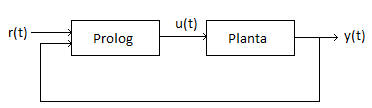
\includegraphics[width=160mm]{Imagens/config1.png}
\end{figure}

Para esta configuração, criou-se regras em prolog para que ele forneça a tensão da bomba de acordo com o nível do segundo tanque, como por exemplo:

\begin{itemize}
\item tanque(N,E):- N<10, E is 4.
\item tanque(N,E):- N>=10, N=<20, E is 2.
\item tanque(N,E):- N>20, E is 0.
\end{itemize}

A segunda configuração, o prolog fornecerá os parâmetros do controlador. no caso, $K_p$, $K_i$ e $K_d$. A figura \ref{segunda configuracao do prolog} mostra o esquema desta configuração.

\newpage

\begin{figure}[ht!]
\caption{segunda configuração do prolog \label{segunda configuracao do prolog}}
\centering
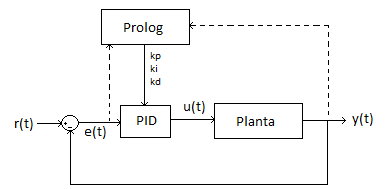
\includegraphics[width=160mm]{Imagens/confg2.png}
\end{figure}

As regras usadas nesta configuração estão descritas a seguir:

\begin{itemize}
\item tanque(E,Kp,Ki):- E=<(-30), Kp is 0.1, Ki is 0.001.
\item tanque(E,Kp,Ki):- E>(-30), E<0, Kp is 1, Ki is 0.01.
\item tanque(E,Kp,Ki):- E>=0, E<30, Kp is 1, Ki is 0.01.
\item tanque(E,Kp,Ki):- E>=30, Kp is 0.1, Ki is 0.001.
\end{itemize}

Nas regras acima, nota-se a ausência do $K_d$. Isso aconteceu porque nos testes, os resultados foram melhores quando $K_d$=0. Logo, ele foi retirado somente para obter um código menor, sem nenhum prejuízo no resultado.


\newpage

%%%%%%%%%%%%%%%%%%%%%% RESULTADOS %%%%%%%%%%%%%%%%%%%%%%%%%%%

\thispagestyle{main}

\section{RESULTADOS}

A biblioteca pyswip facilitou bastante a conexão entre o python e o prolog, já que ela permitia escrever as regras em prolog dentro do código em python.

Para a simulação da primeira configuração, utilizou-se valores de setpoint entre 0 e 20cm. Conforme pode ser visto nas regras para essa configuração, só são permitidos 3 valores de tensão, 0, 2 e 4 volts, dependendo da saída. A figura \ref{10cm} mostra a resposta da planta ao setpoint de 10cm.

\begin{figure}[ht!]
\caption{Resposta da planta para a configuração 1 em 10cm. \label{10cm}}
\centering
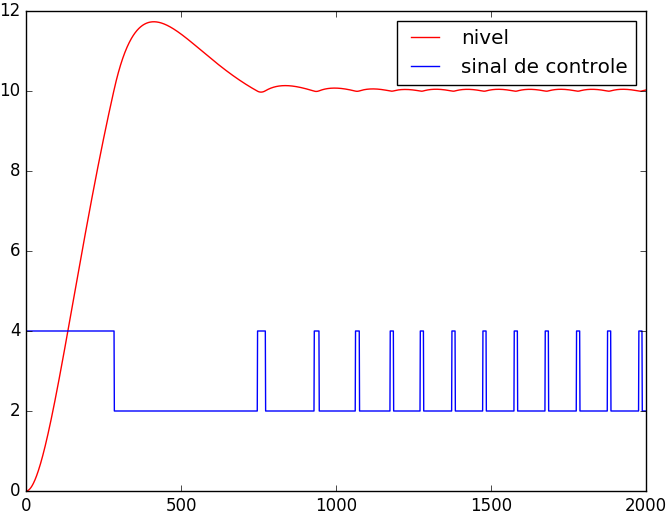
\includegraphics[width=100mm]{Imagens/figure_1_HISTERESE.png}
\end{figure}

Devido ao pouco número de regras, pode ser observado na imagem a mudança brusca do sinal de controle, entre 2 e 4V.

Para simular a segunda configuração, utilizou-se valores de referência entre 0 e 30cm. Primeiro, setou-se a referência em 20cm, obtendo-se o resultado mostrado na figura \ref{10cmc2}.

\begin{figure}[ht!]
\caption{Resposta da planta para a configuração 2 em 10cm. \label{10cmc2}}
\centering
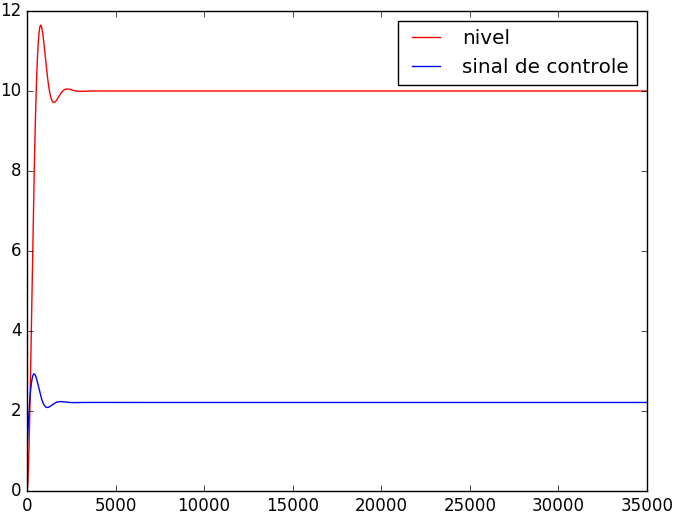
\includegraphics[width=100mm]{Imagens/Figura_Questao2.png}
\end{figure}

Nesta figura, nota-se a boa atuação do controlador, apesar do pouco número de regras implementadas para esta configuração, apenas 4. O regime transitório apresentou pouca oscilação e o erro de regime permanente foi de aproximadamente zero.

Depois, modificou-se o código para que ele alterá-se o setpoint, aleatoriamente, cada vez que o erro fosse menor que 0,000001. O resultado pode ser visto na figura \ref{c2_aleatorio}.

\begin{figure}[ht!]
\caption{Resposta da planta para a configuração 2 com setpoint aleatório. \label{c2_aleatorio}}
\centering
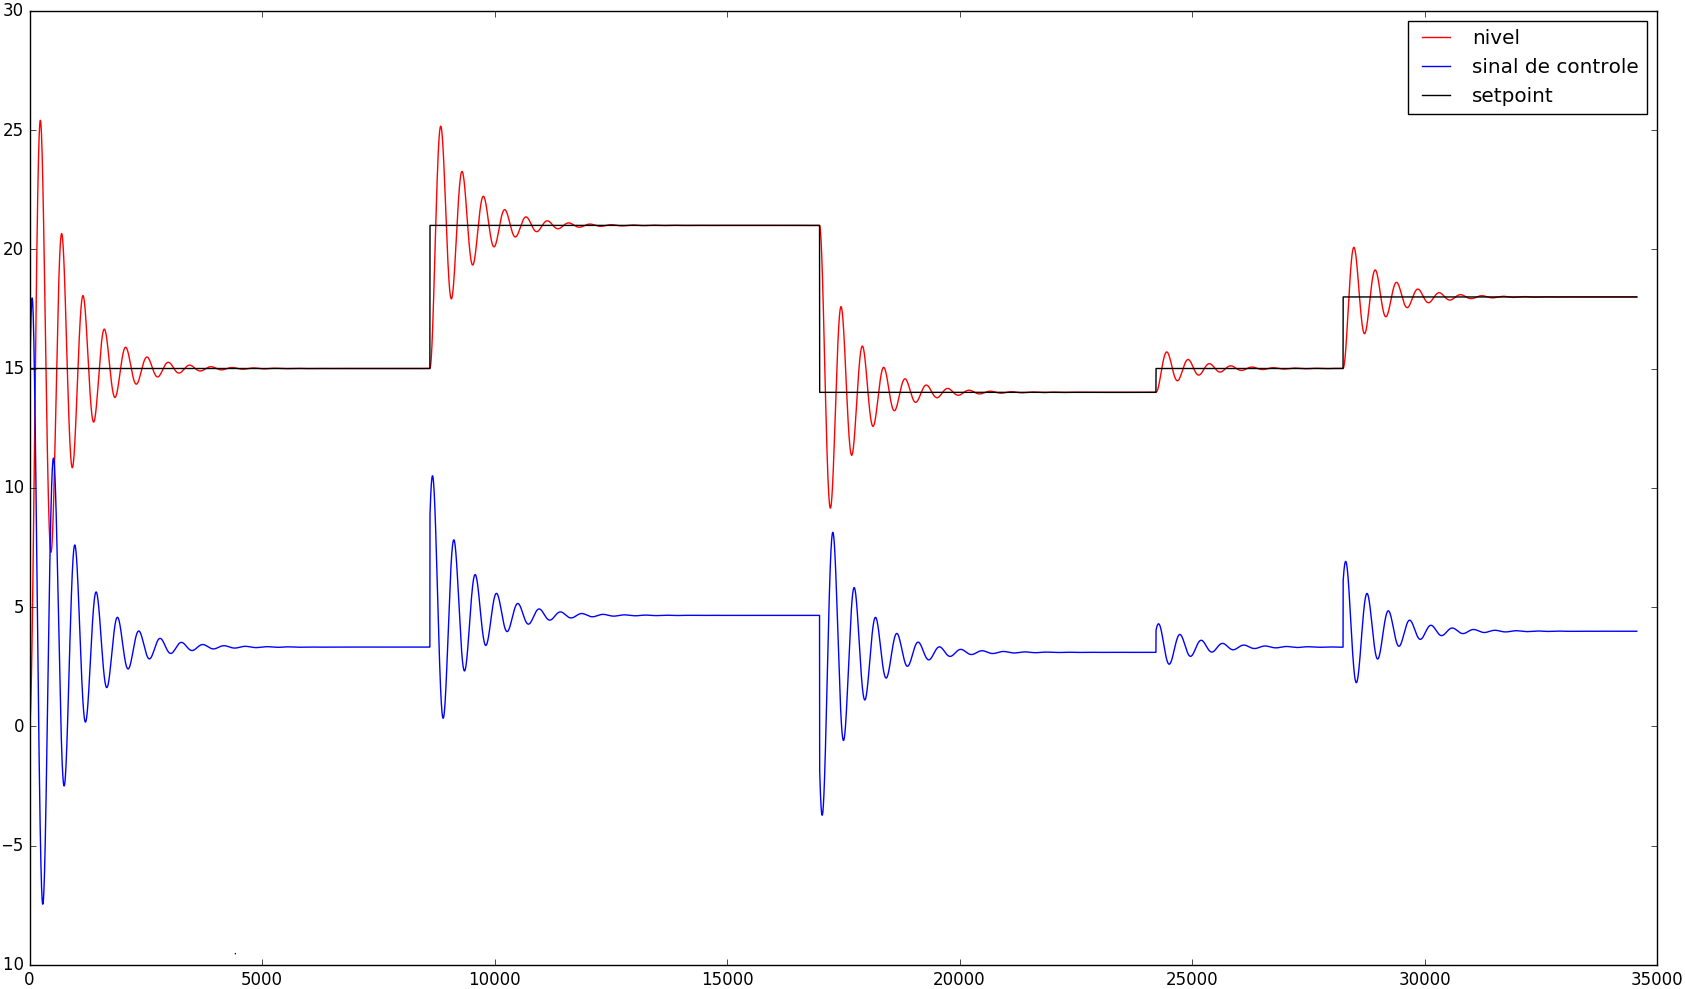
\includegraphics[width=100mm]{Imagens/figure_2_PID.png}
\end{figure}

A planta apresentou uma resposta muito oscilatória no regime transitório. Poderia-se inserir a constante da ação derivativa para reduzir este efeito, porem os resultados mostraram que uma planta pode ser controlada, eficientemente, usando regras em prolog.


\newpage
%%%%%%%%%%%%%%%%%%%%%%% CONCLUSÃO %%%%%%%%%%%%%%%%%%%%%%%%%%%%

\thispagestyle{main}

\section{CONCLUSÃO}

Apesar da estrutura do prolog não parecer tão intuitiva e sequencial como em outras linguagem, como C/C++, python, ela permite que se possa tomar decisões lógicas baseadas em fatos e regras disponíveis. No caso desta simulação, poderia-se analisar algumas situações onde a resposta não foi tão satisfatória e adicionar mais regras para melhorá-las, como por exemplo, aumentar o número de regras para diminuir a variação de tensão da bomba na configuração 1 ou criar regras de valores por faixa de setpoint.  

Esta simulação serviu para mostrar que o prolog é adequado para o controle inteligente de sistemas industriais. Embora não se tenha obtido resultados muito satisfatórios, sejam por falta de tempo para uma melhor sintonia ou pela falta de experiência no uso desta linguagem, ela serviu para implementação prática do que foi abordado em sala de aula.



\newpage

%%%%%%%%%%%%%%%%%%%% REFERÊNCIAS %%%%%%%%%%%%%%%%%%%%%%%%%%%%

\thispagestyle{main}

\section{REFERÊNCIAS}

[1] Apostila da disciplina Paradigmas Programação, Prolog, do Departamento de Engenharia de Computação e Automação – Universidade Federal do Rio Grande do Norte

[2] Apostila da disciplina Sistemas de Controle do Departamento de Engenharia de Computação e Automação – Universidade Federal do Rio Grande do Norte

[3] OGATA, K.: Engenharia de Controle Moderno – 4o Edição, 2003, Prentice-Hall. (OGATA, 2003)

[4] Roteiro do laboratório 1 da disciplina Sistemas de Controle do Departamento de Engenharia de Computação e Automação – Universidade Federal do Rio Grande do Norte

[5] Roteiro do laboratório 5 da disciplina Sistemas de Controle do Departamento de Engenharia de Computação e Automação – Universidade Federal do Rio Grande do Norte

  

% Referências bibliogáficas (geradas automaticamente)
% \addcontentsline{toc}{chapter}{Referências bibliográficas}
% \bibliography{bib/bibliografia}

\appendix

%Apêndice A
\include{apendice}

\end{document}